\documentclass[border=5pt]{standalone}
\usepackage{tikz}
\usepackage{amsmath}
\begin{document}
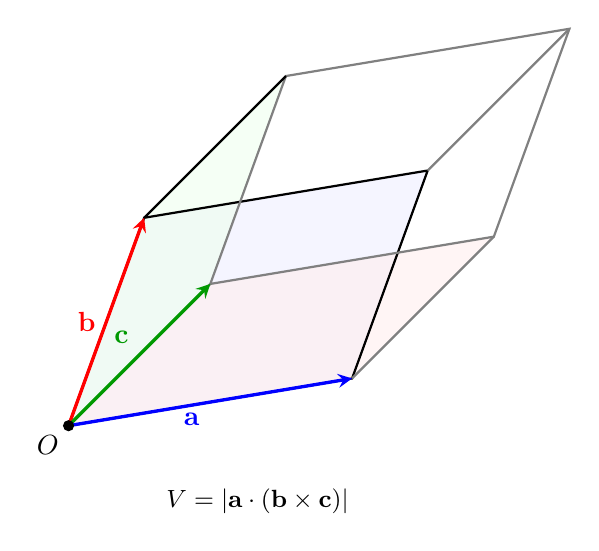
\begin{tikzpicture}[scale=1.2, >=stealth]
  % 3D parallelepiped with vectors a, b, c

  % Front face
  \coordinate (O) at (0,0);
  \coordinate (A) at (3,0.5);
  \coordinate (B) at (0.8,2.2);
  \coordinate (C) at (3.8,2.7);

  % Back face (shifted)
  \coordinate (O2) at (1.5,1.5);
  \coordinate (A2) at (4.5,2.0);
  \coordinate (B2) at (2.3,3.7);
  \coordinate (C2) at (5.3,4.2);

  % Fill faces
  \fill[blue!8, opacity=0.5] (O) -- (A) -- (C) -- (B) -- cycle;
  \fill[red!8, opacity=0.5] (O) -- (A) -- (A2) -- (O2) -- cycle;
  \fill[green!8, opacity=0.5] (O) -- (B) -- (B2) -- (O2) -- cycle;

  % Front face edges
  \draw[thick] (O) -- (A) -- (C) -- (B) -- cycle;

  % Back face edges
  \draw[thick, gray] (O2) -- (A2) -- (C2) -- (B2) -- cycle;

  % Connecting edges
  \draw[thick, gray] (O) -- (O2);
  \draw[thick, gray] (A) -- (A2);
  \draw[thick] (B) -- (B2);
  \draw[thick, gray] (C) -- (C2);

  % Vectors from origin
  \draw[->, very thick, blue] (O) -- (A) node[midway, below left] {$\mathbf{a}$};
  \draw[->, very thick, red] (O) -- (B) node[midway, left] {$\mathbf{b}$};
  \draw[->, very thick, green!60!black] (O) -- (O2) node[midway, above left] {$\mathbf{c}$};

  % Volume formula
  \node[font=\small] at (2, -0.8) {$V = |\mathbf{a}\cdot(\mathbf{b}\times\mathbf{c})|$};

  % Origin
  \filldraw[black] (O) circle (1.5pt) node[below left] {$O$};
\end{tikzpicture}
\end{document}
